% !TeX root = ../thuthesis-example.tex

\chapter{MCP-PMT 的带光强电荷模型}

\section{MCP-PMT 的单光电子电荷模型}
\subsection{MCP-PMT 中的物理过程}\label{sec:mcp-pmt-process}
PMT 的探测效率取决于两个关键因素:QE 系数与 CE 系数。
其中,QE 为 PMT 光阴极发射的光电子与入射光子数的比值,CE 为经过倍增后,阳极收集到的电子数量与入射光电子数量的比值。

为了提高 QE 系数,在 JUNO 中使用的 20 寸 MCP-PMT 具有以下特征:
\begin{itemize}
    \item 上半椭圆球面装配发射光阴极,下半椭圆球面装配反射光阴极,实现接近 $4\pi$ 立体角光电转换范围
    \item 上下具有两块平行的 MCP
\end{itemize}

\begin{figure}
    \centering
    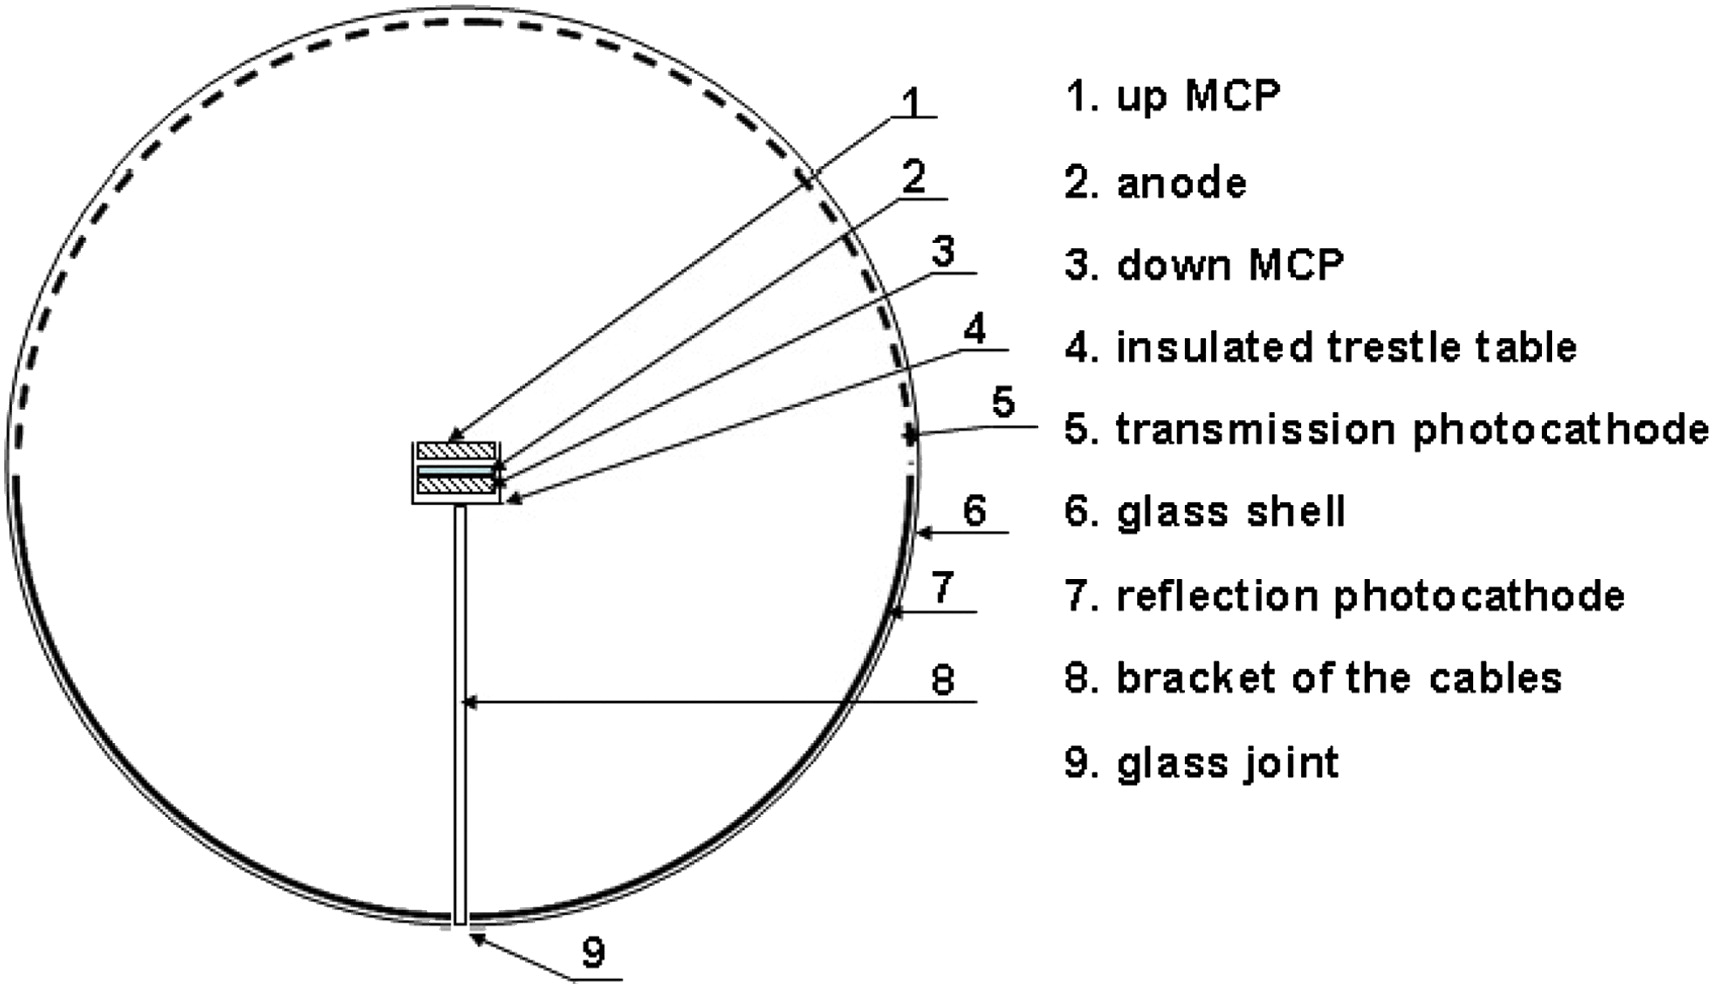
\includegraphics[width=0.75\linewidth]{scheme.jpg}
    \caption{MCP-PMT 的结构设计图\cite{wangNewDesignLarge2012}}
\end{figure}

在光子在 MCP-PMT 内部光阴极与材料发生相互作用产生光电子后,电子在椭圆形玻璃球壳内的电场作用下,向 MCP 迁移。
PMT 需要使用屏蔽线圈来抵消地磁场的影响,使得光电子能以尽量高的效率到达 MCP。
MCP 使用加高压的长通道实现电子加速,并以一定的小角度倾斜,使得电子容易与壁材料发生相互作用实现倍增,
同时又不使二次电子飞行轨迹与壁夹角过大致电子难以逸出。
MCP 的长通道截面积占横截面的比例称为开口比 $A$。

\begin{figure}
    \centering
    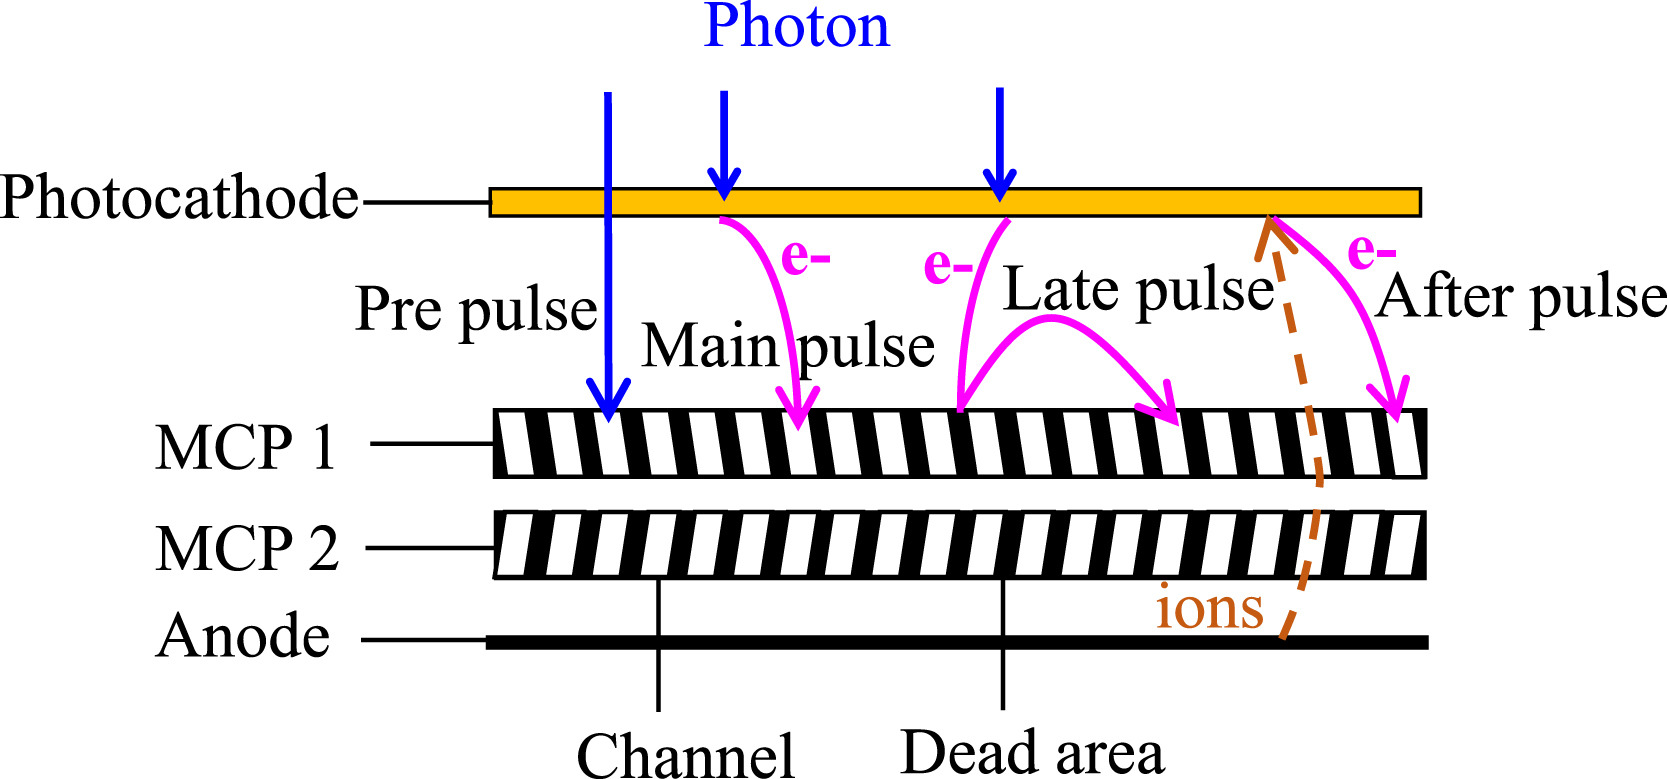
\includegraphics[width=0.85\linewidth]{process.jpg}
    \caption{MCP-PMT 中物理过程\cite{chenPhotoelectronBackscatteringMicrochannel2018}}
    \label{fig:pulses}
\end{figure}

MCP-PMT 的主要噪声来源为离子反馈\cite{MaterialStore2010}。即使 MCP-PMT 需要内部近似真空的工作条件,但仍存余少许的气体分子。
气体分子被电离,在高压电场中与倍增电子运动方向相反,既可能撞击壁产生二次电子被阳极收集,
也可能反向加速直至撞击光阴极,由于从产生到被收集的时间(渡越时间)较电子长,故将与主峰后形成次级脉冲,且还能够对光阴极材料造成损伤。
如果延长加速通道或者提高高压,这些脉冲也将得到放大,为了有效提高信噪比,常常使用两层 MCP 并使通道倾角对称。
由于在正离子与电子运动方向上引入了反角的设计,速度较小的反馈离子更难以进入与产生处对称的另一级 MCP,
从而有效提高信噪比,同时对电子再次倍增,获得较大的增益。

为了提高 CE 系数,最初在 MCP 入射处使用涂层(镍铬电极),使得入射的光电子可能能够在该表面进行倍增。
在后来的设计中,采用了 $\text{Al}_2\text{O}_3-\text{MgO}$ 复合涂层作为 ALD 涂层材料的方案,
起到提高二次倍增电子数 $\delta_{ts}$ 与延长寿命的作用。

在先前基于 Furman 模型\cite{PhysRevSTAB.5.124404}的模拟\cite{chenOptimizationElectronCollection2016}中,将光电子与涂层发生的相互作用分为三类:
\begin{itemize}
    \item 在涂层表面发生弹性散射;
    \item 进入涂层原子,发生散射而脱离涂层;
    \item 与涂层作用产生若干个能量较低的二级电子,亦称为真二次发射电子。
\end{itemize}

\begin{figure}
    \centering
    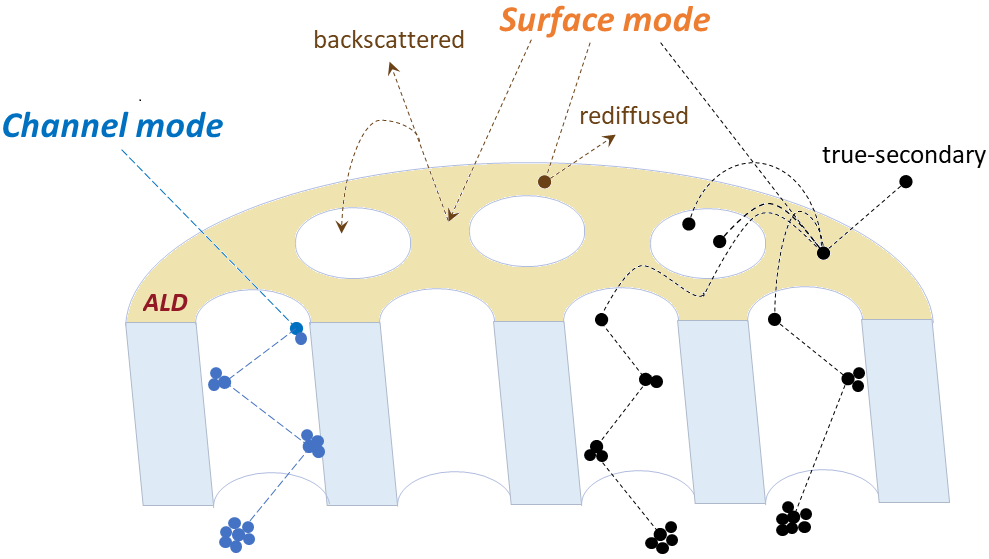
\includegraphics[width=0.85\linewidth]{mcp-pmt.png}
    \caption{光电子与 MCP-PMT 的三种相互作用形式}
\end{figure}

在三种模式中,发生前两种散射模式的单个光电子均只能产生一个光电子,而发生二次倍增的电子则可以产生自然数个真二次发射电子,
其个数 $\delta_{ts}$ 与入射电子能量 $E$、与涂层表面法线夹角 $\theta$ 存在依赖,由 Furman 模型给出:
\begin{equation}
    \delta_{ts}(E,\theta)=\hat{\delta}(\theta)D\left[\frac{E}{\hat{E}(\theta)}\right].
\end{equation}

其中 $\hat{\cdot}$ 代表 $\cdot$ 函数项的极值,$D(\cdot)$ 为一个满足 $D(1)=1,\ D^\prime(1)=0$ 的尺度函数,Furman 等人选择:
\begin{equation}
    D(x)=\frac{sx}{s-1+x^s}.
\end{equation}

其中 $s>1$ 为可调节变量。而对于二次倍增电子数服从的分布,Furman 等人给出了泊松分布与二项式分布两种选择,
其中二项式分布需要依据材料,选择对应的随机变量上限 $M$,在实际未知材料性质的情况下使用泊松分布是更合适的。

\subsection{单光电子电荷响应}\label{sec:spe-charge}
在 8 寸 MCP-PMT 的单光电子电荷响应研究\cite{wengSingleElectronCharge2024}中,电子进孔倍增的电荷响应采用 Gamma 分布描述。
这是因为在每一次倍增中,倍增电子的个数均服从泊松分布,并依次级联,
这种级联泊松最终可以用 Gamma 分布相较于其他常用分布(例如高斯分布)更好地近似。
相较于常用的高斯分布,Gamma 分布的另一个好处是在非正区间上概率密度严格为 0。

同时,真二次发射电子与其他未在涂层表面倍增而进入 MCP 倍增的电子相比,除了能量与到达阳极时间外没有本质区别,
其电荷响应亦使用 Gamma 分布描述。在 8 寸的仿真中,真二次发射电子的电荷被发现服从同一个 Gamma 分布 $\Gamma(\alpha_{ts}, \beta_{ts})$。
在~\ref{sec:mcp-pmt-process} 节中,Furman 模型给出真二次发射电子数目服从泊松分布的建议,因此真二次发射电子的电荷响应部分可以表示为:
\begin{equation}
    \left.
        \begin{array}{c}
        Q_\mathrm{ts}=\sum_{\mathrm{i=1}}^{\delta_{ts}}Q_\mathrm{i}\\
        \delta_{ts}\sim\pi(\lambda)\\
        Q_\mathrm{i}\sim\Gamma(\alpha_{ts},\beta_{ts})
        \end{array}
    \right\}\implies
    Q_\mathrm{ts}\sim\mathrm{Tw}_{\xi}
    \left(\mu(\boldsymbol{\theta_{ts}}),\sigma^2(\boldsymbol{\theta_{ts}})\right),\quad
    \boldsymbol{\theta_{ts}}=(\lambda, \alpha_{ts},\beta_{ts}).
    \label{eq:compound-poisson-gamma}
\end{equation}

即服从泊松分布个数的 Gamma 分布之和等价于指数参数 $\xi\in(1, 2)$ 的 Tweedie 分布。
Tweedie 分布是一种特殊的指数族分布,由 $\xi$ 调节分布的种类,由 $\mu$ 代表期望,由 $\phi$ 线性调节方差:
\begin{equation}
    Y\sim\mathrm{Tw}_{\xi}(\mu, \sigma^2)\implies 
    \left\{
        \begin{array}{c}
        \mathrm{E}[Y]=\mu \\
        \mathrm{var}[Y]=\phi\mu^{\xi}
        \end{array}
    \right.
    \label{eq:tweedie}
\end{equation}

~\eqref{eq:compound-poisson-gamma} 对比~\eqref{eq:tweedie},可得映射关系:
\begin{align}
    \xi & = \frac{2+\alpha_{ts}}{1+\alpha_{ts}}\\
    \mu & = \lambda\cdot\frac{\alpha_{ts}}{\beta_{ts}}\\
    \phi & = (1+\alpha_{ts})\left[\lambda\alpha_{ts}\beta_{ts}^{(1+\alpha_{ts})}\right]^{-\frac{1}{1+\alpha_{ts}}}
\end{align}

对于只在表面弹性散射或进入涂层材料原子核但被散射出涂层的电子,以及没有与涂层相互作用而直接进入 MCP 进行倍增的电子,
它们没有在涂层表面进行倍增,彼此的区别在于飞行径迹与 TT 不同,从而对 TTS 产生贡献。
它们在 MCP 中的倍增行为相同,电荷增益可以使用同一个 Gamma 分布 $\Gamma(\alpha, \beta)$ 来描述。
该分布作为单光电子进入 MCP 倍增的电荷结果,直接表示了 MCP-PMT 对单光电子的增益水平,
因此可以定义增益 $Q_1\equiv\frac{\alpha}{\beta}$ 与分辨率 $\eta\equiv\frac{\sqrt{\alpha/\beta^2}}{\alpha/\beta}=\frac{1}{\sqrt{\alpha}}$。

至此,MCP-PMT 的单光电子响应模型可以表示为:
\begin{equation}
    S(q)=p_0\Gamma(\alpha, \beta)+(1-p_0)\mathrm{Tw}_{\xi}
    \left(\mu(\boldsymbol{\theta_{ts}}),\sigma^2(\boldsymbol{\theta_{ts}})\right),\quad
    \boldsymbol{\theta_{ts}}=(\lambda, \alpha_{ts},\beta_{ts}).
\end{equation}

其中 $p_0$ 代表主峰的占比,它可以认为是所有未在涂层上进行真二次电子发射的原始电子的比例,
它与开口比、进孔比例、涂层材料性质等物理因素直接相关,可以视为级联伯努利事件的概率密度:
\begin{enumerate}
    \item 电子以 $p_{ch}$ 的概率进入 MCP 倍增,以 $1-p_{ch}$ 的概率撞击 MCP 表面 ALD 涂层
    \item 撞击 MCP 上表面的电子以 $p_{ts}$ 的概率进行真二次电子发射,以 $1-p_{ts}$ 的概率进入 MCP 进行倍增
\end{enumerate}

最终可以认为 $p_0=(1-p_{ch})\cdot(1-p_{ts})$。1. 中 $p_{ch}$ 应满足 $p_{ch}<A$,因为存在电场透镜效应,
电场线在平面上的孔隙处呈扩散状,对电子的运动有“发散”的作用,使得电子进入孔隙的概率变小。

8 寸研究中,指出 2. 中有 $p_{ts}\sim90\%$ 且在典型参数下应有 $p_{ts}>75\%$。
依据经验应有 $p_0<A$,关于 MCP-PMT 延迟脉冲的研究\cite{chenPhotoelectronBackscatteringMicrochannel2018}
指出在 $A=65\%$ 的情况下,应有 $p_0=55\%$。

在 8 寸研究中,对真二次倍增电子相对主峰的均值与标准差做出了限制建议:
\begin{align}
    \mu_{ts}&=\frac{\alpha_{ts}}{\beta_{ts}}\in[0.3, 0.7]\ Q_1\\
    \sigma_{ts}&=\sqrt{\frac{\alpha_{ts}}{\beta_{ts}^2}}\in[0.05, 0.3]\ Q_1
\end{align}

本研究中拟合均采取这一建议区间。

\section{分区间数据的拟合方法}
由于一次激光刻度取数中,电荷计数能够达到数万甚至数十万,
直接对每个计数进行拟合的内存消耗与效率极不理想。
如果能够以尽可能接近电荷模型原始概率分布的分区间方式,
将需要计算的计算点减少至数十至数百个,
将有约三个数量级的效率提升。

\subsection{分区间方法}
常用的分区间包括平方根方法、Sturges 公式、Rice 准则、Scott 准则、Terrell-Scott 准则、Doane 公式、Freedman-Diaconis 准则等。

\begin{table}
    \centering
    \caption{多种分区间方法的比较}
    \resizebox{\textwidth}{!}{
    \begin{tabular}{llll}
    \toprule
    方法 & 区间数 & 区间宽 & 优势与适用范围 \\
    \midrule
    平方根方法 & $k=\lceil\sqrt{n}\rceil$ & ------ & 简单 \\
    Sturges 公式 & $k=\lceil\log_2n\rceil+1$  & ------ & \makecell[l]{正态分布;\\样本数量适中} \\
    Rice 准则 & $k=\lceil2\sqrt[3]{n}\rceil$ & ------ & 简单 \\
    Scott 准则 & ------ & $h=\frac{3.49\hat{\sigma}}{\sqrt[3]{n}}$  & \makecell[l]{简单;\\正态分布} \\
    Terrell-Scott 准则 & $k=\sqrt[3]{2n}$ & ------ & \makecell[l]{渐进极小均方误差的积分;\\适用于非正态分布}   \\
    Doane 公式 & \makecell[l]{$k=1+\log_2(n)+\log_2\left(1+\frac{|g_1|}{\sigma_{g_1}}\right)$\\$g_1$偏度,$\sigma_{g_1}=\sqrt{\frac{6(n-2)}{(n+1)(n+3)}}$} & ------ & \makecell[l]{基于 Sturges 公式;\\适用于非正态分布} \\
    Freedman-Diaconis 准则 & ------ & \makecell[l]{$h=2\frac{\mathrm{IQR}(x)}{\sqrt[3]{n}}$\\IQR四分位距} & \makecell[l]{对离群值不敏感;\\适用于非正态分布} \\
    \bottomrule
    \end{tabular}}\label{tab:histogram}
\end{table}

在表~\ref{tab:histogram} 中,Freedman-Diaconis 准则既在系数部分使用了四分位距 IQR,
考虑了随机变量分布的偏度而避免像 Doane 公式一样直接计算偏度与其标准差,降低了计算难度,
又在幂次上同样渐进极小均方误差的积分\cite{freedmanHistogramDensityEstimator1981},
即 $k\propto n^{1/3}\ \simeq\ h\propto n^{-1/3}$,
确保在样本统计量大的情况下能够以最优的幂次还原原始概率分布。
综上所述,本研究中使用 Freedman-Diaconis 准则来对电荷计数进行分区间,再进行拟合。

\subsection{最小二乘法}
不妨约定 $q$ 为自变量,$q_i$ 表示第 $i$ 个直方图区间的自变量闭区间,
$n_i$ 表示第 $i$ 个直方图区间的实际计数,或称为频数,总事例数 $N=\sum_{i}n_i$;
$e_i$ 表示第 $i$ 个直方图区间的预期计数,或称为预期频数,可由下式给出:
\begin{equation}
    e_i(\boldsymbol{\theta}) = N\int_{\inf q_i}^{\sup q_i}\mathrm{d}q\cdot f(q;\boldsymbol{\theta})
\end{equation}

其中 $f(q;\boldsymbol{\theta})$ 代表在给定参数集 $\theta$ 时电荷谱的条件概率密度函数。

将直方图的每一个区间都视为一次测量,测量结果为频数,可以定义 $\chi^2(\boldsymbol{\theta})$:
\begin{equation}
    \chi^2(\boldsymbol{\theta})\equiv\sum_{i}\frac{\left[n_i-e_i(\boldsymbol{\theta})\right]^2}{\sigma_i^2}
    \label{eq:chi-sq}
\end{equation}

其中 $\sigma_i^2$ 代表第 $i$ 个直方图区间的频数的方差。
为了计算方差,使用预期频数 $e_i$ 替代方差 $\sigma_i^2$ 或使用频数 $n_i$ 替代方差 $\sigma_i^2$ 是两种可行的做法。

如果每个区间的计数 $n_i$ 相较总事例数 $N$ 占比小,可以认为渐进总事例数 $N$ 无穷、发生概率 $p$ 无穷小而 $Np$ 有限的泊松分布 $\pi(n_i;Np)$,
因此有近似 $\sigma^2_i=n_i$:
\begin{equation}
    \chi^2(\boldsymbol{\theta})=\sum_{i}\frac{\left[n_i-e_i(\boldsymbol{\theta})\right]^2}{n_i}
    \label{eq:pois-ls}
\end{equation}

如果将每个区间视为各自独立且具有较大数学期望的计数结果,则可近似认为服从高斯分布,
因其误差可以认为仅仅由统计涨落贡献,故具有方差与数学期望相等的特征,
即 $\sigma^2_i=e_i$:
\begin{equation}
    \chi^2(\boldsymbol{\theta})=\sum_{i}\frac{\left[n_i-e_i(\boldsymbol{\theta})\right]^2}{e_i}
    \label{eq:gauss-ls}
\end{equation}

根据大数定律,这两种近似在样本量趋近无穷时,具有相同的极限,但它们在有限样本量下的取舍则有所不同:
\begin{itemize}
    \item~\eqref{eq:pois-ls} 需要每个区间事例数占比都较小;
    \item~\eqref{eq:gauss-ls} 需要每个区间事例数足够多,尤其不能为空,否则不能良定义。
\end{itemize}

在本研究中,发现按照 Freedman-Diaconis 准则划分的直方图中,计数最多的区间计数可达总计数的 20\%,
因此~\eqref{eq:pois-ls} 假设并不成立,且由于每个区间计数较多,
选用~\eqref{eq:gauss-ls} 作为极小化的函数是合适的。

关于拟合结果的误差分析,最准确的办法是对一系列的自变量 $\boldsymbol{\theta}$ 做 Monte Carlo 模拟,
得到 $\chi^2$ 的概率密度分布,从而得到拟合得到 $\chi^2$ 的置信区间,作为该模型的合理性定量依据。
在我们认为每个区间计数较多的前提下,上文已经表明每个区间计数可以认为服从高斯分布,
从而可以近似认为拟合得到的 $\chi^2$ 结果服从卡方分布,得到模型的合理性估计。

\subsection{极大似然法}
同样约定 $q$ 为自变量,$q_i$ 表示第 $i$ 个直方图区间的自变量闭区间,共有 $m$ 个区间,
$n_i$ 表示第 $i$ 个直方图区间的频数,总事例数 $N=\sum_{i}^{m}n_i$,$\boldsymbol{n}=(n_1, n_2, \ldots, n_m)$ 代表各区间的频数向量,
$e_i$ 表示第 $i$ 个直方图区间的预期频数,各区间预期频数使用 $\boldsymbol{e}$ 表示,可由下式给出:
\begin{equation}
    e_i(\boldsymbol{\theta}) = N\int_{\inf q_i}^{\sup q_i}\mathrm{d}q\cdot f(q;\boldsymbol{\theta})
    \label{eq:ei}
\end{equation}

可见存在函数满足参数集 $\boldsymbol{\theta}$ 至预期频数 $\boldsymbol{e}$ 之间的双射。
各区间事例数 $\boldsymbol{n}$ 可以视为总数为 $N$ 的 $m$ 次多项式分布结果,在该处的概率分布密度为:
\begin{equation}
    \begin{aligned}
        P(\boldsymbol{n},\boldsymbol{e}|\boldsymbol{\theta})
        &=P(\boldsymbol{n}|\boldsymbol{\theta})\\
        &=\frac{N!}{n_1!\cdots n_m!}\left[\frac{e_1(\boldsymbol{\theta})}{N}\right]^{n_1}
        \cdots\left[\frac{e_m(\boldsymbol{\theta})}{N}\right]^{n_m}\\
        &=\frac{N!}{n_1!\cdots n_m!}\cdot\frac{\prod_{i=1}^{m}e_i^{n_i}(\boldsymbol{\theta})}{N^N}
    \end{aligned}
    \label{eq:hist-pdf}
\end{equation}

对~\eqref{eq:hist-pdf} 取对数得:
\begin{equation}
    \begin{aligned}
        \ell&=\ln P(\boldsymbol{n}|\boldsymbol{\theta})\\
        &=\sum_{i=1}^{m}n_i\ln{e_i(\boldsymbol{\theta})}
        +\ln{N!}-\sum_{j=1}^{m}\ln{n_j!}-N\ln{N}\\
        &=\sum_{i=1}^{m}n_i\ln{e_i(\boldsymbol{\theta})}+C
    \end{aligned}
    \label{eq:log-l}
\end{equation}

其中 $C$ 代表与自变量 $\boldsymbol{\theta}$ 无关的常数,在极大似然过程中对结果没有影响。
极大似然法相较于最小二乘法,不需要做出近似假设,且对各区间频数 $n_i$ 没有要求,
始终具有良定义,但由于需要计算对数,计算开销更大,在复杂电荷模型的假设下优化更加困难。

\section{傅里叶变换带光强电荷模型}\label{sec:fourier}
出于三个原因,考虑光强的刻度方法有被引入的必要性:
\begin{enumerate}
    \item 在 PMT 的刻度与实际运行中,可能遇到光强较强以至于多个光电子情形不可忽略甚至占主要成分的情况;
    \item 由于本研究所考虑的 MCP-PMT 相较于传统打拿级 PMT,具有电荷长尾的效应,
    实际电荷谱上较主峰能道高的区域由单光电子模型中 Tweedie 成分与多光电子的主峰共同贡献;
    \item 对于低光强的刻度数据,大统计量的 0 电荷计数被排除在单光电子谱刻度外,没有得到充分利用。
\end{enumerate}

拟合引入 0 电荷计数,能够极大提高统计量,得到相对误差较小的光强,
从而在电荷谱的能道较高范围内尽可能消除多光电子的贡献对长尾参数的影响,
提高目标 MCP-PMT 的增益刻度准确性。

\subsection{任意光电子数电荷谱}\label{sec:dft}
光电子个数服从期望为 $\mu$ 的泊松分布,即:
\begin{equation}
    P(\text{PE}=n) = \pi(n;\mu)=\sum_{i=0}^{+\infty}\frac{\mu^{n}}{n!}\cdot e^{-\mu}
\end{equation}

当光电子个数为 0 时,考虑到没有光电子时的电荷应该严格为 0,电荷谱密度可以认为是:
\begin{equation}
    S_{0\text{PE}}(q)=N_{0\text{PE}}\cdot\delta(q)=\pi(0;\mu)\cdot\delta(q)
\end{equation}

当光电子个数为正整数 $k\in\mathbb{N}^{+}$ 时,电荷谱密度等效于 $k$ 个单光电子谱卷积:
\begin{equation}
    \begin{aligned}
        S_{k}(Q = \sum_{i = 1}^{k} q_i ) 
        & = \pi(k;\mu)\cdot\underbrace{
        \int_{-\infty }^{+\infty}\mathrm{d}q_1\cdot S(q_1)
        \cdots \int_{-\infty }^{+\infty}\mathrm{d}q_k\cdot S(q_k)
        }_{k}\\
        &=\pi(k;\mu)\cdot\underbrace{S(q)\otimes\cdots\otimes S(q)}_{k}.
    \end{aligned}
    \label{eq:kpe-charge}
\end{equation}

其中 $S(q)$ 为单光电子电荷谱概率密度函数。傅里叶变换 $\mathcal{F}$ 能够将卷积变为另一个域上的直积:
\begin{equation}
    \mathcal{F}\left[f(t)\otimes g(t)\right]=\mathcal{F}[f(t)]\cdot\mathcal{F}[g(t)].
    \label{eq:fourier}
\end{equation}

因此对~\eqref{eq:kpe-charge} 做傅里叶变换并对 $k\in\mathbb{N}^{+}$ 求和即得正整数个光电子时的电荷谱密度为:
\begin{equation}
    \tilde{S}_{\ge1\text{PE}}(p)=\sum_{k=1}^{\infty}
    \pi(k;\mu)\cdot\tilde{S}^k(p).
    \label{eq:pe-charge}
\end{equation}

其中 $\tilde{\cdot}(p)$ 代表函数 $\cdot$ 经过 $\mathcal{F}$ 后在另一个数域 $\{p\}$ 上的数值。
考虑~\eqref{eq:pe-charge} 补全 0 个光电子时的无穷级数求和:
\begin{equation}
    \begin{aligned}
        \tilde{S}_{\ge1\text{PE}}(p)
        &=\sum_{k=0}^{\infty}\pi(k;\mu)\cdot\tilde{S}^k(p)-\pi(k;\mu)\\
        &=\sum_{k=0}^{\infty}\frac{e^{-\mu}}{k!}\cdot\left(\mu\tilde{S}(p)\right)^k-e^{-\mu}\\
        &=e^{\mu(\tilde{S}(p)-1)}-e^{-\mu}\\
        &=e^{-\mu}(e^{\mu\tilde{S}(p)}-1).
    \end{aligned}
    \label{eq:postive-charge}
\end{equation}

通过傅里叶变换,能够将任意多个光电子的卷积分布转化为另一个定义域上的直积,
并借助泊松分布的性质实现解析求和,既不需要截断无穷级数求和,也不需要计算卷积,
是完全无损失的理论方法,因此得到的参数应是无偏的。

考虑 0 电荷处的概率密度则需要综合考虑 0 个光电子与单光电子中 Tweedie 成分的贡献:
\begin{equation}
    \begin{aligned}
        S_{\text{total}}(q=0)
        &=S_{\ge1\text{PE}}(q=0)+S_{0\text{PE}}(q=0)\\
        &=\sum_{k=1}^{\infty}\pi(k;\mu)\cdot S^k(q=0)+\pi(0;\mu)\\
        &=\sum_{k=0}^{\infty}\pi(k;\mu)\cdot S^k(q=0)\\
        &=\sum_{k=0}^{\infty}\frac{e^{-\mu}}{k!}\cdot\left[\mu S(q=0)\right]^k\\
        &=\sum_{k=0}^{\infty}\frac{e^{-\mu}}{k!}\cdot\left[\mu(1-p_0)e^{-\lambda}\right]^k\\
        &=e^{\mu\left[(1-p_0)e^{-\lambda}-1\right]}.
    \end{aligned}
    \label{eq:zero-charge}
\end{equation}

\subsection{复合 Simpson 数值积分}
借助~\ref{sec:dft} 所述的方法,一组参数已经能够利用 FFT 与 IFFT 映射到一系列采样点上的概率密度函数值。
为了得到原电荷谱上特定区间内的预测频数,需要使用数值积分方法。
常用的数值积分方法包括:矩形法,Lagrange 插值法与 Newton-Cotes 插值法等,
在此不展开介绍各方法的应用场景与变形。

复合 Simpson 积分法是 Newton-Cotes 插值法的特殊形式,特别适用于间隔给定的特定区间上的数值积分。
其具体计算方式如下:
\begin{equation}
    \begin{aligned}
        \int_{a}^{b}f(x) dx
        &=\sum_{i=1}^{n/2}\frac{h}{3}\left[f(x_{2i-2})+4f(x_{2i-1})+f(x_{2i})\right]-\frac{f^{(4)}(\xi_i)}{90}h^5 \\
        &=\frac{h}{3}\left[f(x_0)+4f(x_1)+2f(x_2)+\cdots+2f(x_{n-2})+4f(x_{n-1})+f(x_n)\right]
        -\frac{h^2}{90}\sum_{i=1}^{n/2}f^{(4)}(\xi_i) \\
        &=\frac{h}{3}\left[f(x_{0})+4\sum_{i=1}^{n/2}f(x_{2i-1})+2\sum_{i=1}^{n/2-1}f(x_{2i})+f(x_{n})\right]
        -\frac{h^2}{90}\sum_{i=1}^{n/2}f^{(4)}(\xi_i).
    \end{aligned}
    \label{eq:simpson}
\end{equation}

其中 $x_i$ 为等间距 $h$ 的序列满足 $a=x_0<x_1<\cdots<x_n=b$。
考虑连续函数 $f^{(4)}(\xi)$ 的介值定理,应有:
\begin{equation}
    \frac{2}{n}\sum_{i=1}^{n/2}f^{(4)}(\xi_i)=f^{(4)}(\xi),\quad\xi\in\left[\min(\xi_i), \max(\xi_i)\right].
\end{equation}

依此给出~\eqref{eq:simpson} 的误差项为 $-\frac{nh^5}{180}f^{(4)}(\xi)=-\frac{(b-a)h^4}{180}f^{(4)}(\xi)$,
与原函数的四阶导数成正比,因此当且仅当对于三次及以下多项式,其误差严格为 0,或称为代数精度为 3。

复合 Simpson 积分法只需要使用特定点的函数值,在细分区间较多、每段区间较平滑的函数上,它的表现良好,
因此在本实验中采样点函数值到原电荷谱区间频数的预测均使用复合 Simpson 积分法计算。
为了尽可能减小误差,需要采样点间隔 $h$ 尽可能小。
Freedman–Diaconis 准则给出的区间宽 $h\propto n^{-1/3}$,
对于统计量越大的电荷刻度数据,原电荷谱的分区间数越大、间距越小,复合辛普森积分法效果越好。

\subsection{傅里叶变换的准确度与性能}
计算机并不能够对连续的 $S_{\text{total}}(q)$ 函数进行傅里叶变换,只能够使用有限离散傅里叶变换(Discrete Fourier Transformation,以下简称 DFT)对其进行近似,
并使用逆有限离散傅里叶变换(Inverse Discrete Fourier Transformation,以下简称 IDFT)。
应当从准确度与性能方面进行考量。

DFT 与 IDFT 结合的方法能够在离散距离趋近于无穷小时的极限为连续傅里叶变换与其逆变换,因此当采样间隔足够小时,即可实现理想的近似。
合适的间隔应当由定理~\ref{theo:shannon} 决定:
\begin{theorem}[Nyquist–Shannon 采样定理]\label{theo:shannon}
    对于具有带宽限制(即傅里叶变换后频率在有限区域以外为零)例如频率上限为 $f_s$ 的连续信号,使用周期冲激序列进行采样,
    若要完全还原初始连续信号的信息而不发生混叠,则应以不低于 $2f_s$ 的频率进行采样。
\end{theorem}

在实际中,由于连续函数的傅里叶变换常常不具有带宽限制,可以设定频率阈值下限,只需要满足采样频率至少高于该阈值对应频率的二倍,
原始连续信号的主要信息就能够被还原。在本研究中,将依据 Freedman–Diaconis 准则划分的电荷谱区间继续细分至 32 份后,
再增加区间已经没有可以显著观测的变化,可以认为已经理想地还原了原始连续电荷谱的信息。

快速傅里叶变换(Fast Fourier Transformation,以下简称 FFT,逆算法同理简称 IFFT)是一种 DFT 的高效算法,利用了 DFT 中系数的对称性与周期性,
能够将朴素 DFT 算法的 $O(n^2)$ 时间复杂度降低到 $O(n\log{n})$,对于本研究中每个 MCP-PMT 数万至数十万的统计量表现出显著的优势。

综上所述,傅里叶变换刻度方法的本质优势为避免卷积与无穷级数求和的时间复杂度与精度损失,
而使用较多的采样点,同时满足数值积分、FFT 与 IFFT 准确度的要求,
只需要付出较为廉价的内存代价,是理想的升级。

\section{刻度方法}

\subsection{电荷谱截断预处理}\label{sec:cut}
PMT 中存在部分巨大脉冲,是由 $\mu$ 子穿过 PMT 玻璃时发射的切伦科夫光与天然放射性本底造成的\cite{zhangStudy20inchPMTs2022}。
具体地,根据脉冲幅值,可以将划分为 PMT 的噪声计数主要来源分为三类\cite{zhangDarkCount20inch2024}:
\begin{itemize}
    \item $0\sim10$ mV,主要由热致电子发射(暗噪声)贡献;
    \item $10\sim100$ mV,主要由天然放射性贡献;
    \item $100\sim500$ mV,主要由 $\mu$ 子致切伦科夫光贡献。
\end{itemize}

在实际电荷谱中,除了主要事例(暗噪声、激光等)对应的电荷响应,还存在由 $\mu$ 子与天然放射性本底贡献的电荷,且集中在电荷较大的区域。
由于其对主峰后能道较高区域有贡献,因此需要引入一个电荷谱拟合时的上限截断。

在还原山体、玻璃器材中包含的 $^{238}\text{U}\ /\ ^{232}\text{Th}\ /\ ^{40}\text{K}$ 含量与未灌装水之前的实验条件下,
能够得到模拟结果,如图~\ref{fig:cut} 所示。

\begin{figure}
    \centering
    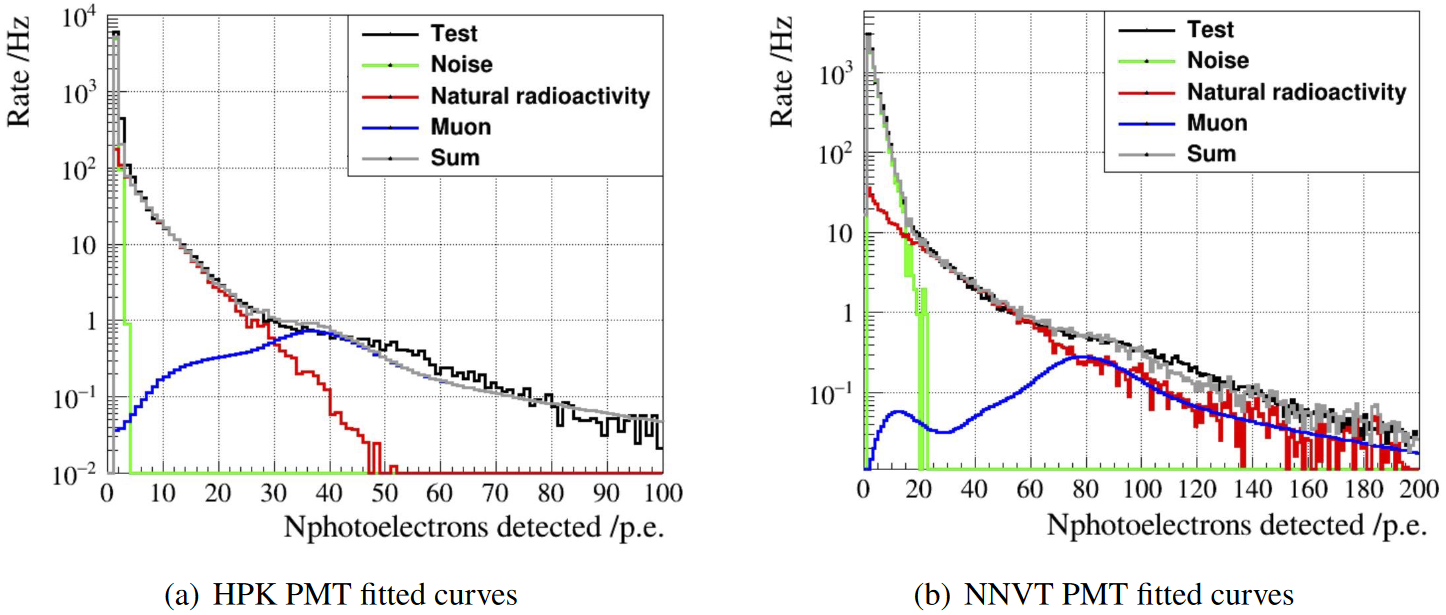
\includegraphics[width=\linewidth]{cut.png}
    \caption{Dynode PMT 与 MCP-PMT 各本底计数率\cite{zhangStudy20inchPMTs2022}}
    \label{fig:cut}
\end{figure}

对于不同的数据集应当采取不同的策略。对于暗噪声采数,暗噪声计数率约 $10\sim50$ kHz,但由于阈值较高(通常有至少 3 个或 7 个或 20 个 PMT 同时过阈才记录波形的设置),
按照暗噪声 50 kHz、偶然符合时间窗 50 ns 的假设进行估计,四重及以上偶然符合计数率有 $f_{coin}\ll1\enspace\text{Hz}$,实际触发率较低,
因此暗噪声的电荷计数主要由三重及以下符合贡献。
依据图~\ref{fig:cut} 可认为在 4 倍单光电子(photoelectron 或 PE)水平下暗噪声触发率接近其他本底的 20 倍左右,可以认为成分较为单一。

对于激光等光源采数,例如 OSIRIS 现场激光刻度触发率为 1.5 kHz,单脉冲的期望水平为 $\mu=0.01$ PE\cite{junocollaborationDesignSensitivityJUNO2021},
对于~\ref{sec:osiris} 节中位于赤道平面上的激光调制位于 $75\%\sim78\%$ 强度,光电倍增管平均光子探测效率为 29.1\%\cite{JUNOPhysicsDetector2022},
可以估计单激光通道下 PMT 接受 PE 频率期望为 3.3 Hz,即 PE 光子数服从强度为 3.3 的时齐泊松过程,
这与现场单激光通道采数 $\sim2\times10^{3}\enspace\text{PE}\ /\ 12\enspace\text{m}$ 的采数率符合。
此时暗噪声也属于本底,但信噪比相较暗噪声采数仍较优,此时预计 5 PE 较为合适。

已经完成的模拟研究中对于 PMT 工作环境的考虑并不完全,仍然需要考虑灌装水与灌装液体闪烁体后的其他本底水平。
灌装后水能够进一步屏蔽周围岩石、玻璃的放射性传播,因此天然放射性项在已经灌装水的探测器中影响将被削弱。

液闪中的 U/Th 等元素及其衰变链的活度受到严格控制,但在循环过程中会引入氡,经过 3 次液体闪烁体循环后,
OSIRIS 内部 $^{214}\text{Bi}-^{214}\text{Po}$ 特征事例的事例率 $\sim2\times10^{-3}\enspace\text{Hz}\ /\ 20\enspace\text{m}^3$ 
升至 $\sim1\times10^{-1}\enspace\text{Hz}\ /\ 20\enspace\text{m}^3$,
在 OSIRIS 探测器中相较于激光刻度采数的频率有 30 倍差距,但在 JUNO 中央探测器中这一比例将更微弱,
因此尤其是 JUNO 中央探测器需要在液体闪烁体循环后氡几乎消耗殆尽时再进行激光采数。

本研究中使用 OSIRIS 的激光刻度数据,综合考虑各本底,选取较简单的 5 倍主峰截断来近似 5 倍 PE 截断。

\subsection{评价指标}\label{sec:criterion}

定义自由度 ndf 为数据点数与模型参数个数之差,对于样本来自于高斯分布的情况,$(\chi^2,\text{ndf})$ 服从卡方分布:
\begin{equation}
    p(\chi^{2},n)=\frac{1}{2^{n/2} \Gamma(n/2)}[\chi^{2}]^{n/2-1}e^{-\chi^{2}/2},\quad0\leq\chi^{2}\leq\infty 
    \label{eq:chi-distribution}
\end{equation}

该种方法称为卡方检验,适用于拟合性检验与独立性检验。
特别地,在 $n\rightarrow\infty$ 时,$\chi^2$ 趋近于自由度为 $n-1$ 的卡方分布。
基于 $\alpha$ 显著性水平,定义 $\chi_\alpha^2$ 为关于 ndf 的临界函数,作为检验的卡方依据。

对于拟合性检验,存在更直接的指标:$\chi^2/\text{ndf}$。~\eqref{eq:chi-sq} 指出 $\chi^2$ 代表数据点偏差平方与方差的比值,
它与自由度 ndf 的比值代表平均意义上每个自由度拟合的相对偏差,在数据点较多的情况下也可近似为每个数据点拟合的相对偏差。
一般可以认为 $\chi^2/\text{ndf}\le1$ 为极优的拟合,$\chi^2/\text{ndf}=3\sim5$ 为较好的拟合。
